\documentclass[12pt,man,hidelinks]{apa7}

\setlength {\marginparwidth }{2cm}
\usepackage[english]{babel}
\usepackage[utf8]{inputenc}
\usepackage{amsmath}
\usepackage{graphicx}
\usepackage[colorinlistoftodos]{todonotes}
\usepackage[justification=centering]{caption}
\usepackage[style=apa]{biblatex}
\usepackage{csquotes}
\addbibresource{references.bib}

\let\oldquote\quote
\let\endoldquote\endquote
\renewenvironment{quote}[2][]
  {\if\relax\detokenize{#1}\relax
     \def\quoteauthor{#2}%
  \else
     \def\quoteauthor{#2~---~#1}%
  \fi
  \oldquote}
  {\par\nobreak\smallskip\hfill\quoteauthor%
  \endoldquote\addvspace{\bigskipamount}}

% Ignore everything above this line. You should only really need to edit this document below this line.

\title{\large{Insert Project Title Here}}
\shorttitle{Project Title LastName}
\author{First Last}
\affiliation{American University}
\note{\today}

\begin{document}
\maketitle

I recommend that before you get started hacking away on your term paper you spend the thirty minutes to read through the introduction to \LaTeX~that Overleaf has put together \footnote{\url{https://www.overleaf.com/learn/latex/Learn_LaTeX_in_30_minutes}}. However, if you absolutely must dive straight in, the information in this document should suffice to help you see the basic structure for the fundamental commands you will need to write a term paper. You can copy and paste many of the commands as they are present here and change only what is necessary for your own paper.

\section{A Section Heading} 
Much like Markdown, you need two new lines to start a new paragraph. You can cite something like this~(\cite{Abril07}), by using the cite command and the name of the reference~(\cite{JCohen96}). The references will be correctly formatted and alphabetized at the end of the document~(\cite{Cohen07}). You can cite multiple authors at the same time like this~(\cite{Abril07, Cohen07}). Only the items that have been cited will appear in the references section at the end. Luckily, Overleaf will make it easy for you to reference anything that you have placed in the references.bib file through auto-complete suggestions. 

\subsection{A Subsection Heading}

This can make it a little easier to get started on an outline. Think about what evidence you need to start, and where, and put together an itemized list of sections and subsections. You can create itemized lists in \LaTeX~like this:

\begin{itemize}
    \item I think I'll talk about patents first by citing \cite{Abril07}
    \begin{itemize}
        \item Sub item - I'll say something about patents.
        \item Then I'll say something about dilemmas
        \item Then finally, I'll talk about trolling. \todo{research trolling}
    \end{itemize}
    \item Then I'll talk about Digital libraries by citing~\cite{JCohen96}.
    \begin{itemize}
        \item I'll need to reference Figure \ref{fig:boat}
    \end{itemize}
\end{itemize}

All references are placed in the references.bib file\footnote{I am okay with you putting \textit{some} things into footnotes rather than full sources in the bib. Online articles you cite as evidence need a reference. For corporate websites, tools, services, etc. a simple footnote to the URL is fine with me.}. A secondary system called BibLaTeX is responsible for reading the information there and creating beautifully formatted reference sections for you. BibTeX formatted entries can be created directly from Google Scholar, and there are many online generators to help you structure them (e.g., Zotero\footnote{\url{https://zbib.org/}}). The point here is that you do not have to worry about styling and moving your references around by hand. Get as much information as you can find about your source into the references.bib entry, and LaTeX will do the work of styling and organizing your references for you.

If you need to put a big quote into the text, it is useful to set it apart from the rest by using the quote command. Notice that you need to use two single quotes, and you have to be specific about start quotes and end quotes. The left single quote is on the tilde key near your left pinky finger, and the right single quote is on the double quote key near your right pinky finger. \LaTeX~treats double quotes differently - "I have no good answer for why it does this." This is but one of the potential surprises in \LaTeX~syntax. While the introductory document and this paper go over many of the basics, see the Roberts article for more information on some of the ``gotchas''~(\cite{Roberts}).

\begin{quote}{\cite{JCohen96}~(not really, but this is where the author goes)}
``Lorem ipsum dolor sit amet, consectetur adipiscing elit. Sed sem mauris, lobortis at mattis et, feugiat a neque. Vestibulum eget sagittis mi, ac ultrices neque. Fusce dictum dui ut risus tempus mollis. Ut scelerisque euismod mattis.''
\end{quote}

\section{Another Section Heading}

You can add pictures if you like, and reference them in the text. Give each figure a custom label, then you can reference the figure by the label and \LaTeX~will handle the ordering. The APA format will automatically place them at the end of your document. Here's a picture of a boat~(Figure \ref{fig:boat}). You may notice that there are tilde \textasciitilde~characters in the \LaTeX~source document that do not appear in the rendered version. These are typically placed between text that describes a reference and the command that creates the reference. \textasciitilde~in LaTeX is a special symbol that will force a non-breaking space between the left and right text.

\begin{figure}
\centering
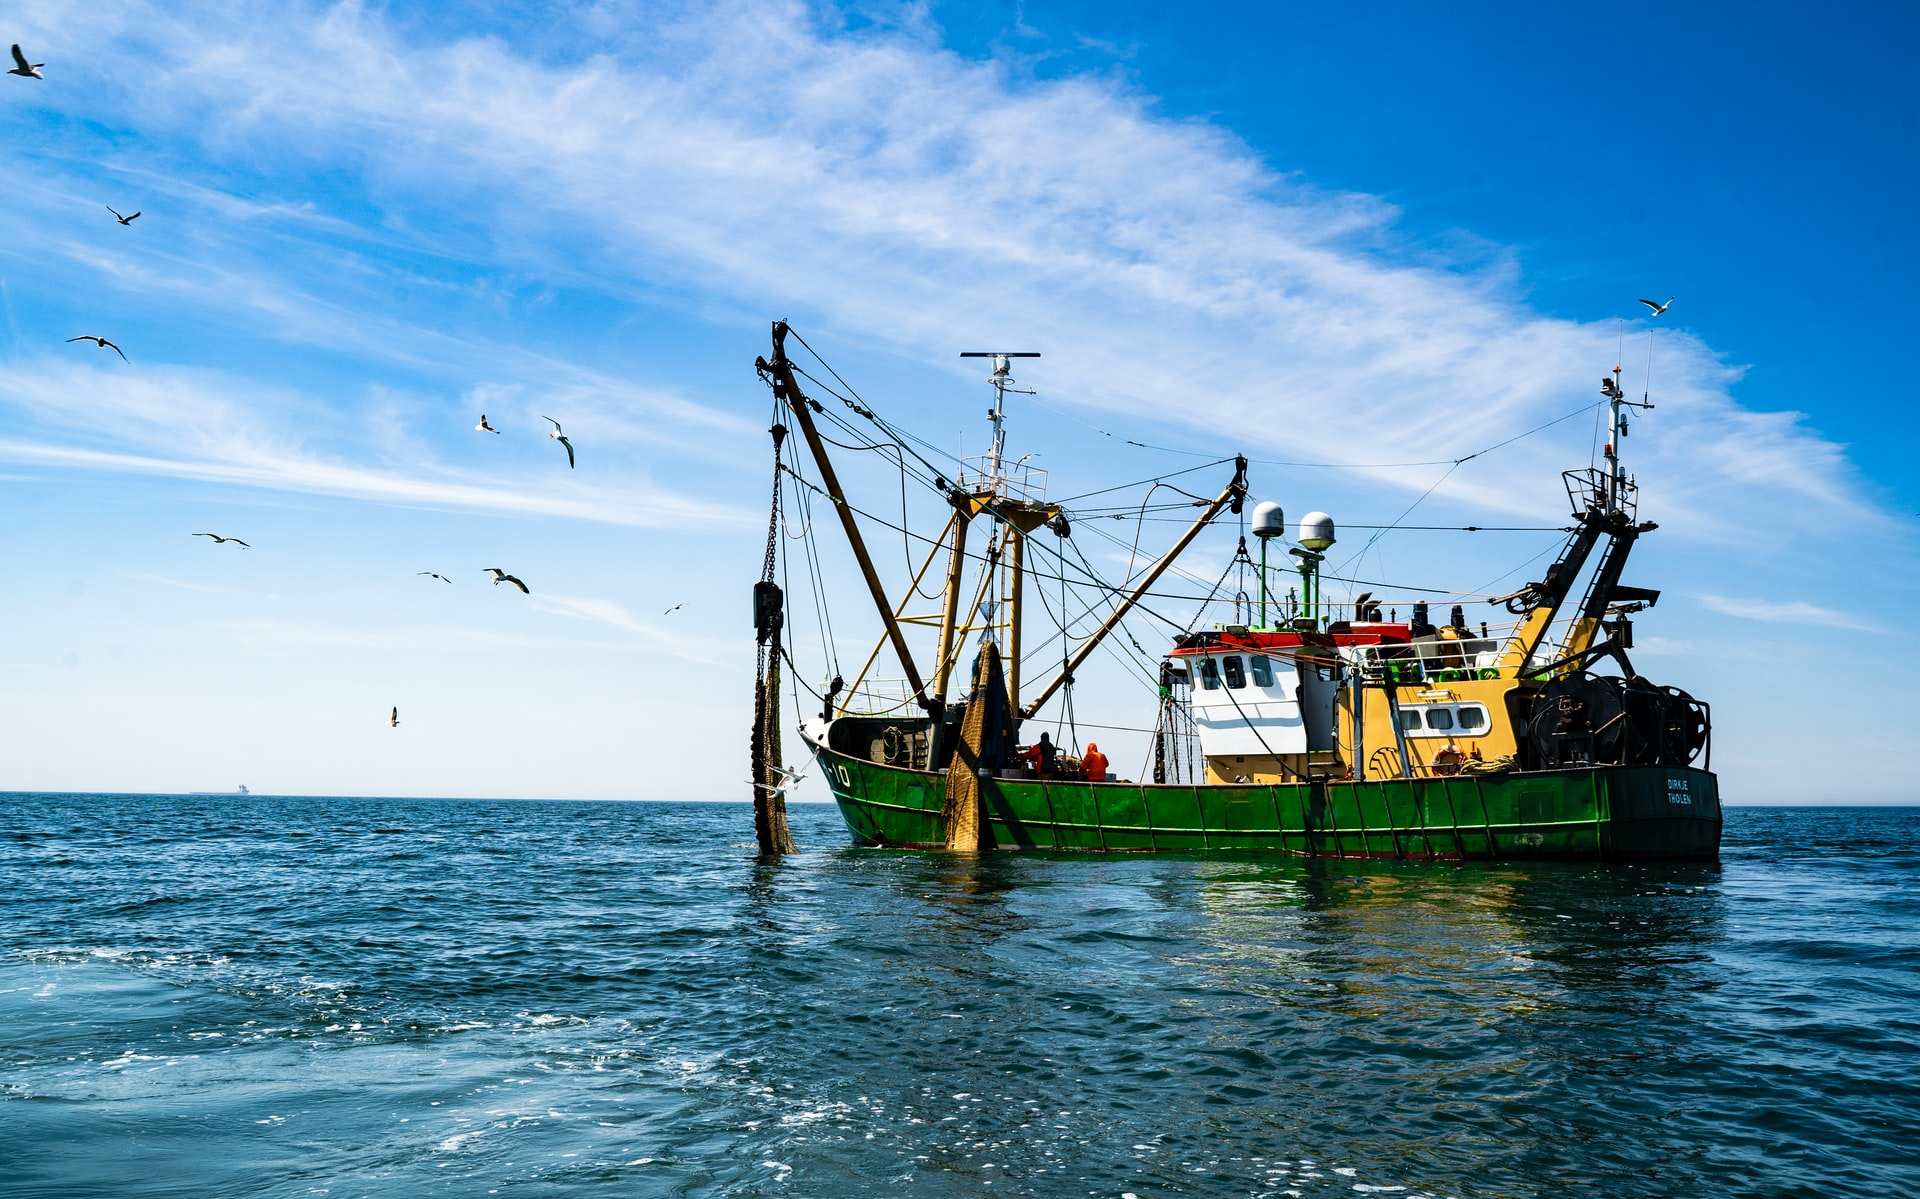
\includegraphics[width=0.75\linewidth]{img/trawler.jpg}
\caption{Boats are neat.}
\label{fig:boat}
\end{figure}

You can potentially include tables if you want, but it is unlikely that you will need to do so for this course. They are somewhat complicated~(Table \ref{Tab:Tcr}), but can be referenced in the text using a label much like a figure. I would recommend that if you absolutely must include a table, you use an online Table Generator\footnote{\url{https://www.tablesgenerator.com}} to create one automatically. Still, keep it as simple as possible.

\begin{table}[ht]
\caption{My Table}
\centering
  \begin{tabular}{l l}
    material  & T [K]\\
    \hline
    Sn                     & 3,7 \\
    Pb                     & 7,2 \\
    Al                     & 1,2\\
  \end{tabular}
  \label{Tab:Tcr}
\end{table}


\printbibliography

% \bibliographystyle{apalike}
% \bibliography{references}

\end{document}
